\begin{center}
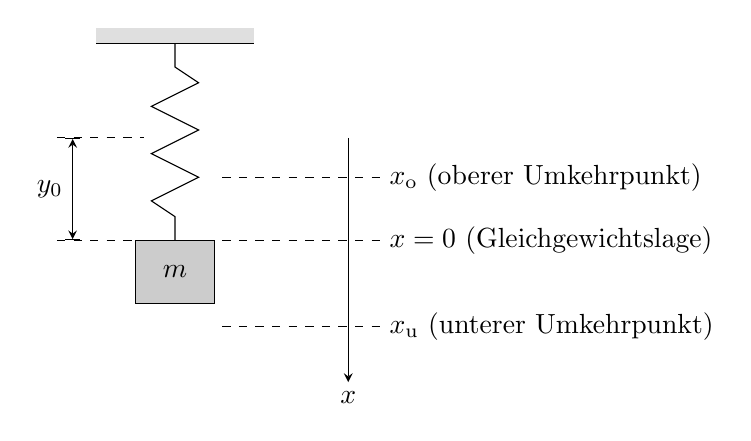
\begin{tikzpicture}[>=stealth]
 \fill[gray!25] (-1,0) rectangle (1,0.2);
 \draw (-1,0) -- (1,0);
 \draw (0,0) -- (0,-0.3) -- (0.3,-0.5) -- (-0.3,-0.8) -- (0.3,-1.1) -- (-0.3,-1.4) -- (0.3,-1.7) -- (-0.3,-2.0) -- (0,-2.2) -- (0,-2.5);
 \draw[fill=gray!40] (-0.5,-2.5) rectangle (0.5,-3.3);
 \node at (0,-2.9) {$m$};
 \draw[dashed] (-1.5,-1.2) -- (-0.4,-1.2);
 \draw[|<->|] (-1.3,-1.2) -- (-1.3,-2.5) node[midway, left] {$y_0$};
 \draw[dashed] (-1.5,-2.5) -- (-0.5,-2.5);
 \draw[dashed] (0.6,-1.7) -- (2.6,-1.7) node[right] {$x_\mathrm{o}$ (oberer Umkehrpunkt)};
 \draw[dashed] (0.6,-2.5) -- (2.6,-2.5) node[right] {$x = 0$ (Gleichgewichtslage)};
 \draw[dashed] (0.6,-3.6) -- (2.6,-3.6) node[right] {$x_\mathrm{u}$ (unterer Umkehrpunkt)};
 \draw[->] (2.2,-1.2) -- (2.2,-4.3) node[below] {$x$};
\end{tikzpicture}
\end{center}
In der Gleichgewichtslage ist die Feder um $y_0$ gedehnt, und die Federkraft hält der Gewichtskraft das Gleichgewicht:
\begin{align}
 k\,y_0 &= m\,g
\end{align}
Die Auslenkung $x$ wird von der Gleichgewichtslage aus nach unten gemessen. Bei der Auslenkung $x$ ist die Feder um $y_0+x$ gedehnt, und die Masse liegt um $x$ tiefer als in der Gleichgewichtslage. In den Umkehrpunkten ist die kinetische Energie null, die Gesamtenergie besteht also aus Spannenergie und potentieller Energie (Nullniveau in der Gleichgewichtslage):
\begin{align}
 E &= \frac{1}{2}k\left(y_0+x\right)^2 - m\,g\,x \\
   &= \frac{1}{2}k\,y_0^2 + \left(k\,y_0-m\,g\right)x + \frac{1}{2}k\,x^2 \\
   &= \frac{1}{2}k\,y_0^2 + \frac{1}{2}k\,x^2
\end{align}
Der lineare Term fällt wegen $k\,y_0 = m\,g$ weg. Weil die Energie erhalten bleibt, gilt für die beiden Umkehrpunkte
\begin{align}
 \frac{1}{2}k\,y_0^2 + \frac{1}{2}k\,x_\mathrm{o}^2 &= \frac{1}{2}k\,y_0^2 + \frac{1}{2}k\,x_\mathrm{u}^2 \quad\Rightarrow\quad x_\mathrm{o}^2 = x_\mathrm{u}^2
\end{align}
Da die beiden Umkehrpunkte verschieden sind, folgt $\result{x_\mathrm{o} = -x_\mathrm{u}}$: Sie liegen gleich weit oberhalb bzw. unterhalb der Gleichgewichtslage. \hfill $\square$
